\section{Dashboard}
L' header del Dashboard è uguale come struttura per ogni tipologia d'utente dove troviamo un pulsante di modifica dei dati 
personali chiamato profilo e il logout (esci).



\subsection{Struttura}
    Questa sezione serve per definire i termini con cui chiamare gli elementi che compongono la pagina dell'applicazione.
    Componenti principali:
    \begin{itemize}
        \item Barra del menu;
        \item {Sidebar}\ped{G};
        \item Contenuto della pagina;
        % \item Footer.
    \end{itemize}

    \begin{figure}[H]
        \centering
        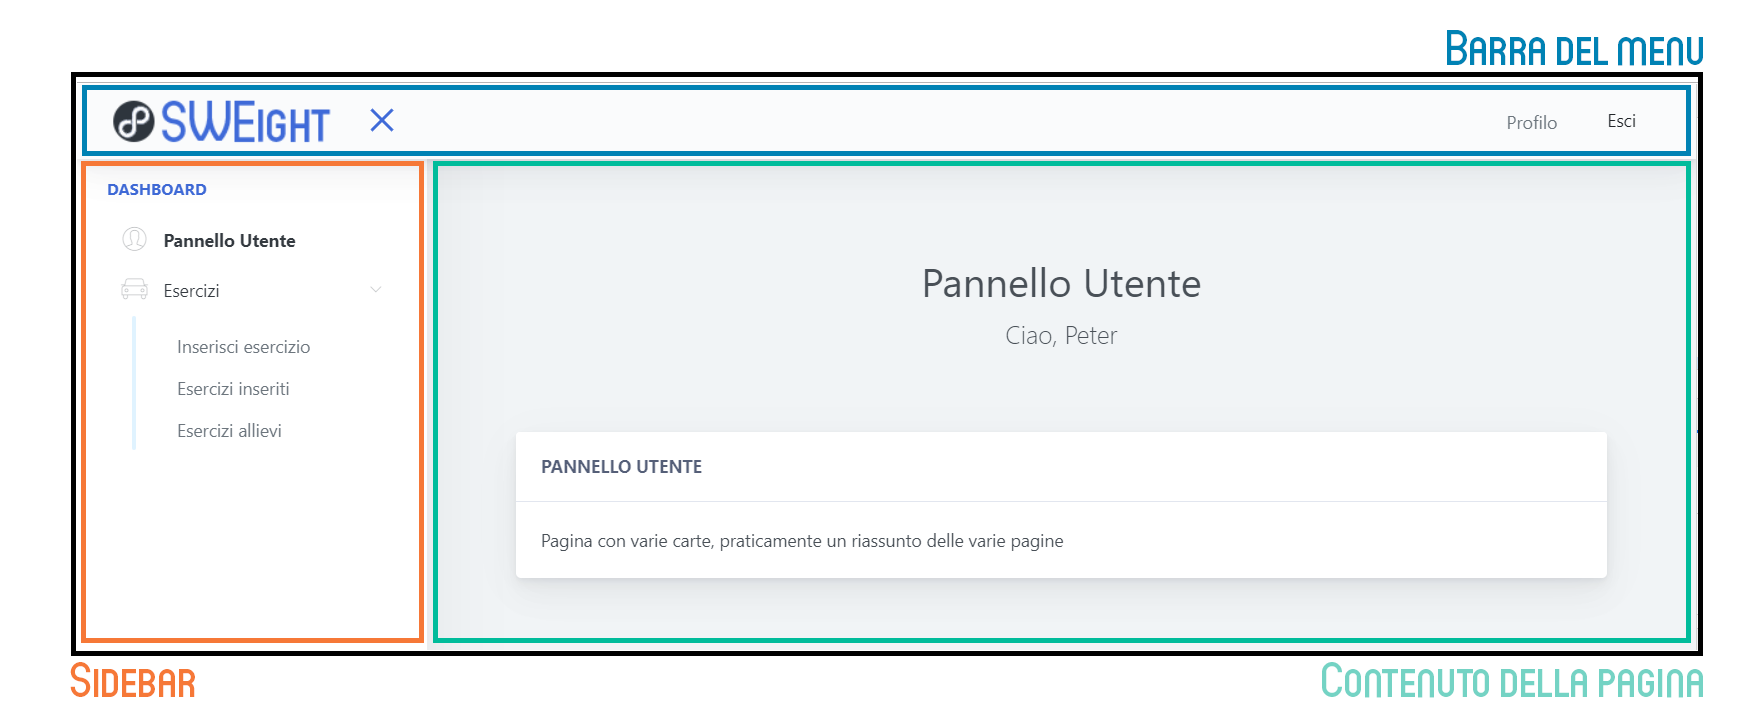
\includegraphics[width=17cm]{sez/img/istruzioni/dashboardMod.png} 
        \caption{Svolgimento esercizio}\label{fig:1}
    \end{figure}
\newpage

\subsection{Autenticazione}
    \subsubsection{Registrazione}
    Se non si è ancora registrati è possibile farlo cliccando sul button \textit{registrati} presente nella barra del menu.
    Una volta compilato il form sarà possibile accedere alla piattaforma come utente autenticato.
    Se si sceglie come ruolo \textit{sviluppatore} sarà necessario attendere una conferma da parte dell'amministratore prima di poter 
    accedere.
    I dati sono tutti obbligatori e la form visualizzata sarà la seguente.
    \begin{figure}[H]
        \centering
        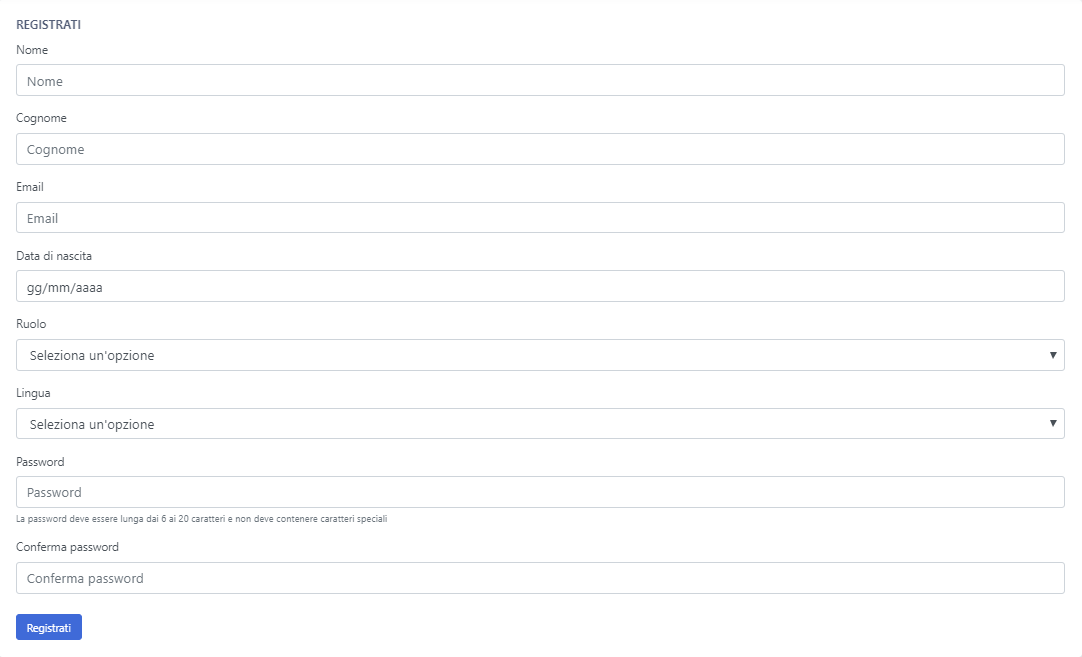
\includegraphics[width=1\linewidth]{sez/img/autenticazione/formRegistrazione.png} 
        \caption{Form per la registrazione}\label{fig:1}
    \end{figure}

    \subsubsection{Login}
    Dopo aver effettuato la registrazione si accede cliccando su \textit{accedi} nella barra del menu.
    Si accede inserendo email e password.
    \begin{figure}[H]
        \centering
        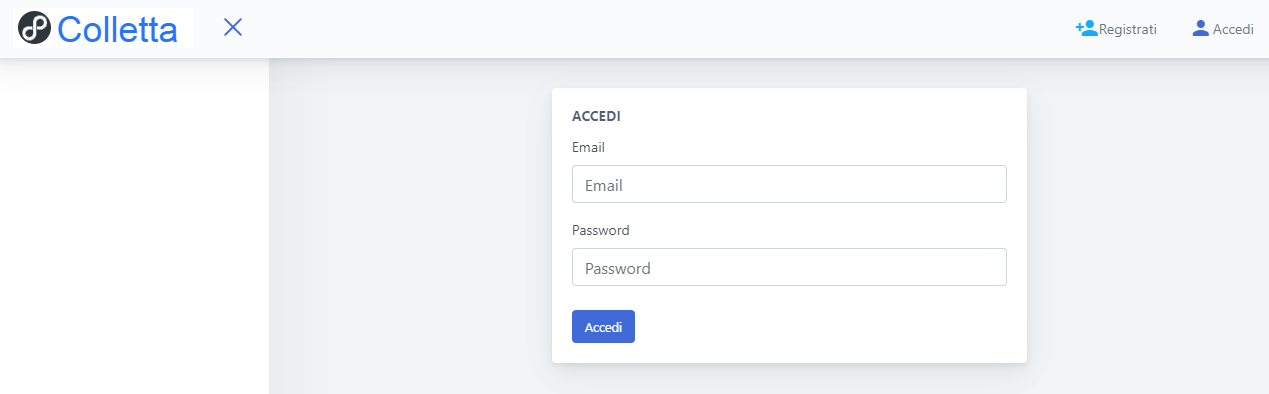
\includegraphics[width=1\linewidth]{sez/img/autenticazione/formAccedi.png} 
        \caption{Dati per effettuare l'accesso}\label{fig:1}
    \end{figure}

    \subsubsection{Logout}
    Per effettuare il {logout}\ped{G} si deve cliccare su la voce \textit{Esci} dalla barra del menu. Esso permette all'utente  di finire la propria sessione.
    \newpage

% UTENTE AUTENTICATO
\subsection{Utente autenticato}

    \subsubsection{Studente}
    Lo studente è l'utente che può svolgere esercizi, con correzioni
    automatiche oppure con correzioni degli insegnanti.
        \paragraph{Sidebar} \mbox{}\\ \\
            La sidebar dello studente presenta le seguenti voci:
            \begin{itemize}
                \item Pannello utente;
                \item Esercitazione libera;
                \item Compiti per casa;
                \item Esercizi svolti;
                \item I tuoi voti.
            \end{itemize}
            % \begin{figure}[H]
            %     \centering
            %     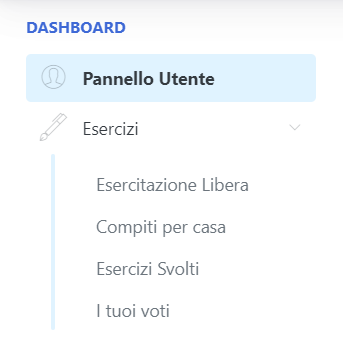
\includegraphics{sez/img/studente/sidebarStudente.png} 
            %     \caption{sidebar dello stidente}\label{fig:1}
            % \end{figure}
        \paragraph{Pannello utente}\mbox{}\\ \\
        SCREEN NON DISPONIBILI
        Il pannello utente è un riassunto di tutti i progressi e le attività
        svolte dallo studente.
        \paragraph{Esercitazione libera}\mbox{}\\ \\
        In questa sezione si svolge l'esercizio inserendo nel form la frase che 
        si preferisce. Se la frase non è stata inserita da nessun insegnante la 
        correzione sarà generata automaticamente.
       \\ Svolgimento:
        \begin{enumerate}
        
            \item Scrivi la frase che vuoi analizzare dentro al form;
            \item Clicca su \textit{svolgi esercizio};
            \item Svolgi l'esercizio e clicca \textit{completa}.
        \end{enumerate}
        \begin{figure}[H]
                \centering
                \includegraphics[width=17cm]{sez/img/studente/EsercitazioneLiberaEsegui.png} 
                \caption{sidebar dello stidente}\label{fig:1}
        \end{figure}
        \newpage
        \paragraph{Compiti per casa}\mbox{}\\ \\
        SCREEN NON DISPONIBILI
        In questa sezine è possibile visualizzare gli esercizi che sono
        stati assegnati dall'insegnante.
        \paragraph{Esercizi svolti}\mbox{}\\ \\
        SCREEN NON DISPONIBILI
        In questa sezione è possiblie visualizzare gli esercizi che sono
        già stati svolti.
        \paragraph{I tuoi voti}\mbox{}\\ \\
        SCREEN NON DISPONIBILI
        In questa sezione è possibile visualizzare i voti....

    \subsubsection{Insegnante}
    L'insegnante è l'utente che può inserire esercizi e assegnarli.
        \paragraph{Sidebar}\mbox{}\\ \\
        La sidebar dell'insegnante presenta le seguenti voci:
        \begin{itemize}
            \item Pannello utente;
            \item Inserisci esercizio;
            \item Esercizi inseriti;
            \item Esercizi allievi.
        \end{itemize}
        \paragraph{Pannello utente}\mbox{}\\ \\
        SCREEN NON DISPONIBILI
        Il pannello utente è un riassunto di tutti i progressi e le attività
        svolte dallo studente.
        \paragraph{Inserisci esercizio}\mbox{}\\ \\
        Questa sezione da la possibilità all'insegnante di inserire un esercizio.
        \begin{figure}[H]
            \centering
            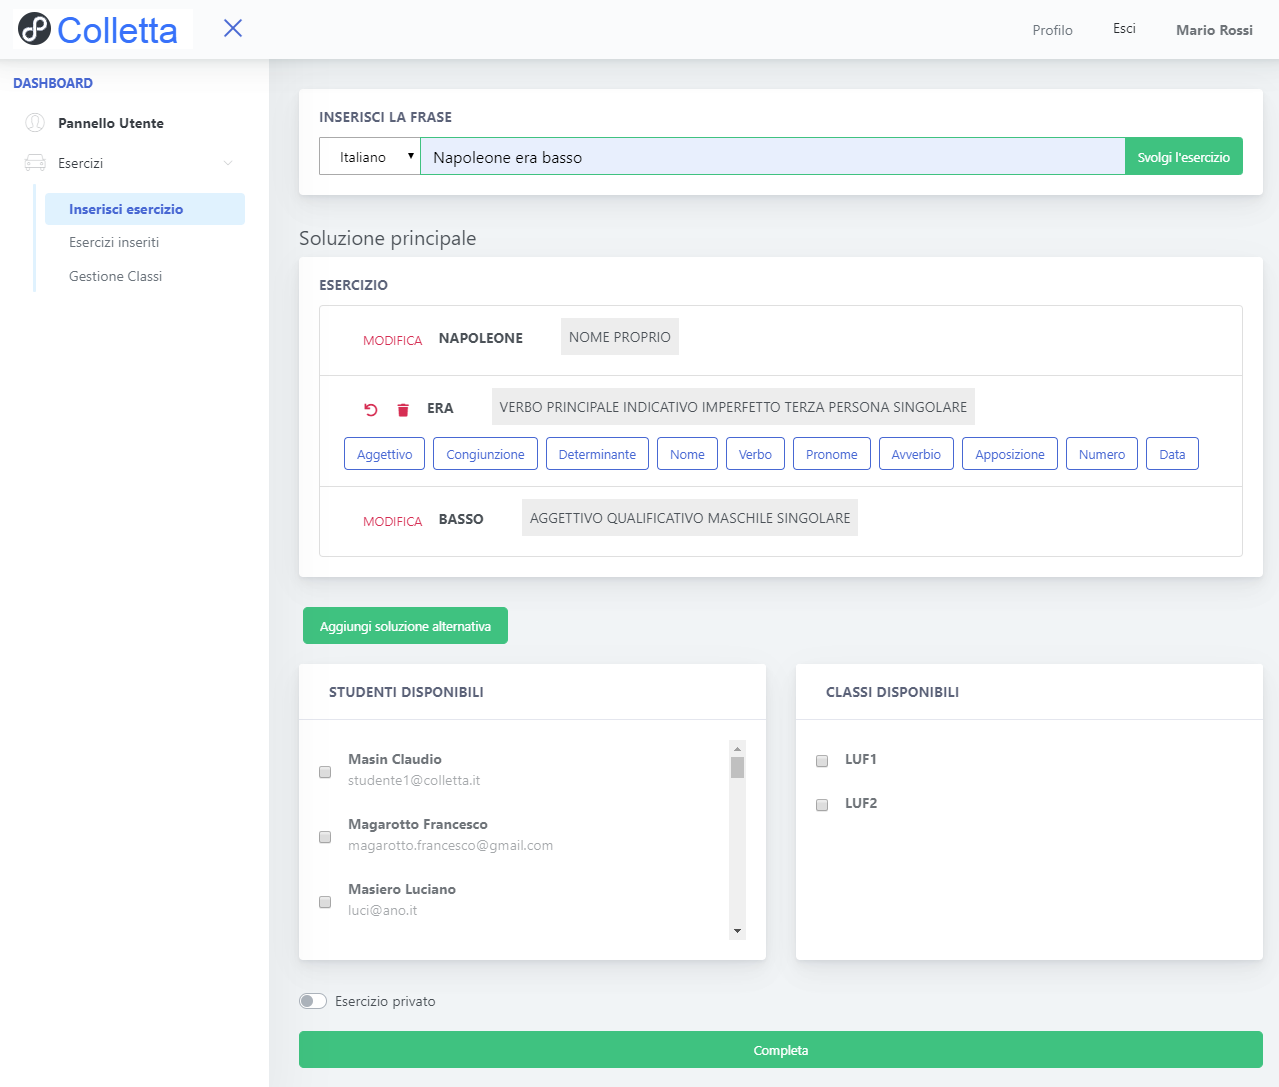
\includegraphics[width=17cm]{sez/img/insegnante/inserisciEsercizio.png} 
            \caption{Insegnante: Inserisci esercizio}\label{fig:1}
        \end{figure}
        Dopo aver inserito la frase e aver cliccato svolgi esercizio verrà visualizzata
        la correzione automatica. Se ritenuta errata c' è la possibilità di modificare la 
        soluzione cliccando su \textit{modifica}.
        \paragraph{Esercizi inseriti}\mbox{}\\ \\
        SCREEN NON DISPONIBILI
        Questa sezione permette di visualizzare tutti gli esercizi inseriti
        \paragraph{Esercizi allievi}\mbox{}\\ \\
        SCREEN NON DISPONIBILI

    \subsubsection{Sviluppatore}
    
    \paragraph{Sidebar}\mbox{}\\ \\
    La sidebar dello studente presenta le seguenti voci:
    \begin{itemize}
    \item Pannello utente;
    \item Pannello sviluppatore.
    \end{itemize}
    \paragraph{Pannello utente}
    \paragraph{Pannello sviluppatore}
    
\subsubsection{Amministratore}
\paragraph{Sidebar}
Breve guida per l'amministratore:
\begin{itemize}
\item conferma richiesta sviluppatore;
\item elimina allievo;
\item elimina insegnate.
\end{itemize}
\subsubsection{Content}
